\chapter{Глава 7}

В прошлой части мы дошли до одного из поворотных пунктов в судьбе Японии – Вашингтонской конференции 1921-1922 годов, достаточно подробно поговорили о внешнеполитических и внутриполитических раскладах в Империи Восходящего солнца, обозначили первоначальное отношение к международному форуму бывших союзников и перечислили состав японской делегации. Наконец, мы порассуждали на тему отношения Британии к своему японскому союзнику, причинах, которые побудили англичан “сдать” японцев, а также последствиях этого шага.

Теперь же настало время плотно взяться непосредственно за Конференцию – её ход и итоги. Но прежде стоит затронуть весьма важный вопрос: почему Япония, вполне сознающая, что в Вашингтоне будут приниматься невыгодные для неё решения, и сомневающаяся только в степени их невыгодности (весьма сильно последнюю недооценивая), не могла просто отказаться от участия в ней? В первую очередь, конечно, причина в неведении – если бы в Токио заранее знали, насколько серьёзными будут потери по итогам Конференции, то никогда не стали бы официально направлять туда делегацию. Во вторых, сыграл свою роль опыт Парижской конференции, которая, с одной стороны, прошла для Империи Восходящего солнца вполне успешно, а с другой продемонстрировала прецедент китайского демарша, которым Поднебесная не только ничего не добилась, но ухудшила своё положение. Наконец, Конференция была весьма умело обставлена американской дипломатией. Официально она дополняла Версаль, с целью упрочить мир в не слишком затронутом положениями итогового документа Парижской конференции Азиатско-Тихоокеанском регионе. Венцом же должно было стать подписание договора о так называемой Дальневосточной, или Тихоокеанской Антанте – союзе сколь широком, столь и виртуальном, недейственном. Формой союзнического участия даже в случае прямой агрессии против другого члена альянса были, как прямо будет сказано в тексте подписанного 13 декабря 1921 договора – к слову, первого принятого документа Конференции, были “взаимные консультации”. Решительно никаких конкретных обязательств. Но демонстративный отказ от участия в Вашингтонской конференции, а значит и в проектируемой Дальневосточной Антанте был равносилен тому, чтобы самому себе на лбу написать крупными красными буквами “Я – агрессор”.

Штаты позаботились о том, чтобы создать колоссальную шумиху в прессе перед началом переговоров. Вообще Конференция должна была стать беспрецедентно открытой – в существенно большей степени, чем даже Парижская. Любая неточность и нечёткость в дипломатических шагах могла немедленно стать достоянием буквально всего мира, пожелай того дирижёры происходящего – американцы. Не говоря уже о том, что в принципе в японской традиции потеря лица – недопустимая вещь, это создавало бы предпосылки для того, чтобы все те, кто не желал иметь дело напрямую с японской дипломатией, в частности китайцы, могли попытаться перевести прежние двусторонние договорённости в область международной дискуссии, потому что они были заключены под давлением страны, которая теперь саботирует всеобщее движение к прочному миру… Япония была вполне обоснованно уверена, что Китай попытается использовать любую возможность, чтобы освободиться из её удушающих объятий, а потому считала более правильным заранее все эти возможность исключить через диалог с великими державами – в первую очередь США, так же заинтересованными в делах Поднебесной. Ну не понимал никто в Токио, что диалог просто не состоится, а будет диктат! Во многом потому, что, всё же, на Конференцию, как ей казалось, Япония идёт не одна, а с весьма мощным союзником.

Впрочем, определённые ветры уже витали в японском воздухе. По мере приближения Конференции всё больше жителей Японских островов могли бы, повторяя слова героев известной серии фильмов, сказать: “У меня очень нехорошее предчувствие”. Эти веяния дошли и до уровня относительных низов японского общества, достигли они и людей, от природы имевших неустойчивую психику. Одним из них, судя по всему, был и Коничи Накаока – скромный железнодорожный служащий, стрелочник, 19 лет отроду, а ещё – убийца премьер-министра Японии Хара Такаси. 

\begin{figure}[h!tb] 
	\centering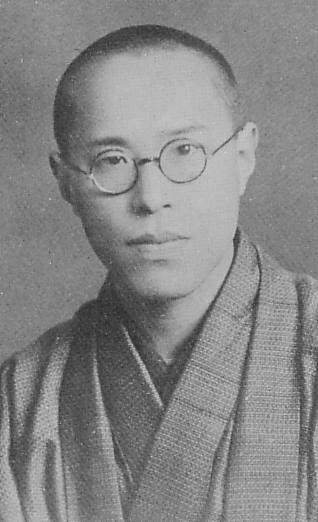
\includegraphics[scale=0.5]{Glava7/dTIP8624ZiE.jpg}
	%	\label{fig:scipion} % Unique label used for referencing the figure in-text\end{document}
	%	%\addcontentsline{toc}{figure}{Figure \ref{fig:placeholder}} % Uncomment to add the figure to the table of contents%----------------------------------------------------------------------------------------
	\caption{Коничи Накаока}%	CHAPTER 2
\end{figure}

В некоторых справочниках можно прочитать, что причиной совершения преступления было недовольство ходом Вашингтонской конференции. Это очевидно неверно – достаточно элементарного знания хронологии, чтобы понять – Накаока зарезал ножом свою жертву 4 ноября 1921, в то время как Вашингтонская конференция началась лишь 12 числа того же месяца. Опять таки, иногда можно видеть фразы вроде “убийство было совершено правым радикалом”. Это верно и неверно одновременно. Накаока никогда не был членом какой-либо политической партии или организации, не имел ясно выраженной идеологической позиции. Фактически молодой парень находился под влиянием своего непосредственного начальника, пожилого работника ж/д станции Токио, Эйдзёро Хасимото, тоже не разу не политика, а просто ворчливого старика, который мог часами рассуждать на тему, общее направление которой вполне сводится к “раньше трава была зеленее”, только с некоторым политическим подтекстом. Убивать кого бы то ни было Хасимото тоже не приказывал. Одним словом, это и близко не похоже на заговор правых террористов, который рисует воображение, и которые будут иметь место в истории Японии позднее. Правыми токийские железнодорожники могут быть названы только по той причине, что вещи, вызывавшие особое недовольство Хасимото, в основном соответствовали правой повестке: партийный кабинет, как уступка после Рисовых бунтов, перемены в культурной жизни и даже всё большая эмансипация женщин. Ну а Вашингтонская конференция была лишь “последней каплей”. Наиболее интересно здесь иное — факт, что к началу ноября 1921 даже железнодорожный стрелочник понимал, что Японию в столице Соединённых Штатов не ждёт ничего хорошего.

О том, насколько Накаока был в действительности политически безграмотен, свидетельствует то, что на допросе в полиции убийца в качестве главной причины своего деяния заявил, что Такаси нарушал конституцию, но когда эти обвинения перешли в конкретную плоскость, то выяснилось, что перечисленные Накаокой эпизоды вполне соответствовали правилам и нормам основного закона Империи. И, тем не менее, ему хватило этого и рассказов старика, чтобы вогнать нож в спину премьер-министра. Ещё одним свидетельством психической нестабильности Накаоки можно считать то, что когда он вышел из тюрьмы по амнистии 13 лет спустя, в 1934, уже в совершенно другой Японии, он отправился в Манчжурию, где… в 1937 обратился в ислам под влиянием татар, мигрировавших ранее из Советской России! Каких только зигзагов не выделывают человеческие судьбы!

Как бы там ни было, но в самый неподходящий момент – прямо на старте Конференции в Японии произошёл правительственный кризис. Если бы и правда существовал заговор, то, быть может, это было бы полбеды – имелись бы люди, которые знали бы о том, что готовится, и могли бы продумать некую программу действий. В действительности гибель Такаси стала для всех полной неожиданностью. ИО премьера временно был назначен министр иностранных дел Итида Косай, исполнявший эти обязанности до 13 ноября. 

\begin{figure}[h!tb] 
	\centering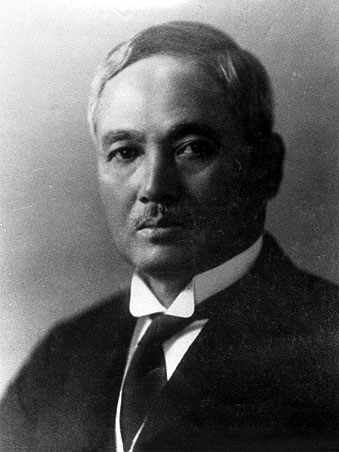
\includegraphics[scale=0.5]{Glava7/d68MMABuGZw.jpg}
	%	\label{fig:scipion} % Unique label used for referencing the figure in-text\end{document}
	%	%\addcontentsline{toc}{figure}{Figure \ref{fig:placeholder}} % Uncomment to add the figure to the table of contents%----------------------------------------------------------------------------------------
	\caption{Итида Косай}%	CHAPTER 2
\end{figure}

И неизвестно даже что хуже – то, как убийство прежнего главы кабинета сказалось на его работе, или то, как оно сказалось на японской дипломатии, главе которой приходилось с полной отдачей заниматься совершенно другими вещами. Новым премьер-министром стал Такахаси Корэкиё. Опытный и талантливый финансист и хозяйственник, бывший в 1911-1913 годах главой национального банка, а после пятикратно в разное время возглавлявший министерство финансов Японии, он очень хорошо проявит себя в годы Великой Депрессии, но в конце осени 1921 это был явно не лучший выбор. Корэкиё не имел никогда дела ни с дипломатической, ни с военной сферами, что в условиях идущей Конференции было большим минусом. Фактически премьер с характерным прозвищем Колобок получил кресло в первую очередь как новый глава партии Риккэн Сэйюкай, в прежней логике партийного кабинета. 

\begin{figure}[h!tb] 
	\centering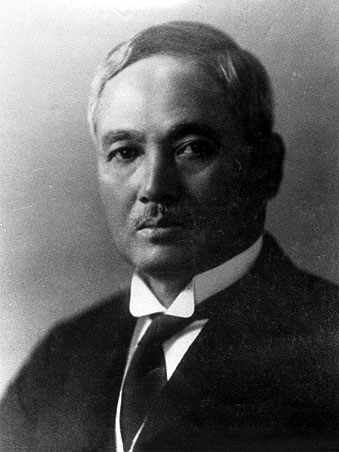
\includegraphics[scale=0.5]{Glava7/d68MMABuGZw.jpg}
	%	\label{fig:scipion} % Unique label used for referencing the figure in-text\end{document}
	%	%\addcontentsline{toc}{figure}{Figure \ref{fig:placeholder}} % Uncomment to add the figure to the table of contents%----------------------------------------------------------------------------------------
	\caption{Итида Косай}%	CHAPTER 2
\end{figure}


А в Вашингтоне тем временем наметился первый страшный удар. Формально стран-участниц было 14: США, Великобритания, Япония, Франция, Италия, Китай, Бельгия, Нидерланды и Португалия, а также отдельно пять британских доминионов. Но реально все переговоры велись Большой тройкой – американцы, британцы и японцы. И уже на первых заседаниях этого неформального коллектива обозначилась неготовность Великобритании действовать как настоящий союзник Японии. Что ещё хуже, сделалось ясно, что ещё до начала Конференции и вообще без японцев, США и Британия уже достигли договорённостей по принципиальным вопросам, которые теперь предполагают только претворить в жизнь, при минимальной корректировке. Когда 13 декабря был подписан договор о Тихоокеанской Антанте, предполагавший признание ничтожными всех ранее заключенных союзов, теоретически японцы и англичане могли бы продолжать действовать сообща и без юридически обязывающих на это документов. И Страна Восходящего солнца хотела бы этого. Но Лондон уже сделал стратегический выбор в пользу Америки. Во всех дальнейших переговорах Япония была предоставлена сама себе и должна была действовать в одиночку против единого фронта всех тех стран, которые были реально заинтересованы в Конференции: Штатов, Великобритании с доминионами и Китая. Последней попыткой переиграть уже проигранную партию здесь была идея всё же придать некий реальный импульс Дальневосточной Антанте, где Англия и Япония могли бы сохранять союз и совместно оказывать влияние на США и их позицию. Но было уже поздно.

Далее события развивались по нарастающей – от плохого к ещё худшему. Началось обсуждение принятого в итоге 6 февраля 1922 года наиболее известного документа Конференции – Вашингтонского морского соглашения.

О том, почему Британия пошла на ограничения морских вооружений – совершенно невиданный для неё шаг, просто непредставимый в XIX столетии, мы поговорили в прошлой части. Франция и Италия были объективно серьёзно истощены войной, так что были бы вполне рады паузе в военно-морском строительстве при том условии, что процесс будет обоюдным и к нему присоединяться и другие. Для США вопрос был в первую очередь средством достижения политического компромисса с Великобританией и давления на всех остальных, и главным образом – Японию. Примечательно, что альтернатива задавалась очень жестко – или Соглашение, или немедленное начало дредноутной гонки вооружений, где неминуемо скажется общее экономическое превосходство США. Для Японии вопрос о флоте тоже был важен не столько сам по себе: ни Китай, ни Советская Россия и близко не обладали ВМС, способными угрожать Японским островам, а другие страны, вроде бы как, пока как противники не рассматривались, хотя конкуренция с флотом США началась уже с середины 1910-х, сколько политически. Это был вопрос о готовности подчиняться.

Очень важно понимать, что Вашингтонское Морское соглашение было составлено как бы из двух частей. Первая, более известная – абсолютные ограничения типов судов по тоннажу. 35000 тонн для линкора, 21000 - для авианосца, 10000 – для любого другого типа надводного корабля, кроме военно-транспортного. Фактически в качестве крайних были взяты размерения крупнейших существующих кораблей. Стандартное водоизмещение британских дредноутов Куин Элизабет – 29 200 тонн, американских типа Колорадо - 32693 тонны, японских типа Нагато - 34 273,2 тонны. Т.е. действительно предлагалось взять паузу, сохранить достигнутый уровень. Правда здесь был свой нюанс, невыгодный для Японии. В нормальной ситуации, по мере увеличения тоннажа и в целом величины новых дредноутов оставалось бы всё меньше верфей, которые могли бы их строить – буквально по паре штук даже в самых развитых морских государствах. Меньший тоннаж существенно увеличивал их число. Если верфи Кобэ и Куре были на самом высоком мировом уровне, то других, способных хоть как-то строить линкоры, в Японии просто не было. В Соединённых Штатах же и Великобритании, как нетрудно догадаться, дела обстояли иначе. В итоге при одновременном старте в случае конфликта мощные судостроительные производства британцев, и, что особенно важно, американцев, могли начать строить дредноуты гораздо более быстрыми темпами и в больших количествах, нежели японские. Стоит добавить, что сохранилась эта проблема и позднее: уже годы спустя после заключения Соглашения, Япония вынужденно пыталась реализовывать концепцию “меньше (в смысле количества), да лучше”, которую в полной мере она попыталась воплотить в проекте линкоров Ямато.

Но кроме ограничений тоннажа по типам было и ещё кое-что. Вторая часть Соглашения устанавливала документально закреплённые соотношения силы флотов ведущих стран Земного шара. Для Британии и США оно предполагалось равным, а для всех остальных – по нисходящей и выглядело следующим образом:

США и Британская империя (включая доминионы) 525 000 тонн максимального тоннажа, или 3

Япония 315 000 тонн максимального тоннажа, или 1,75

Франция и Италия 175 000 тонн максимального тоннажа, или 1

Для достижения заданных цифр необходимо было как вывести из состава флотов действующие корабли, так и отказаться от строительства новых. По странам утилизировались:

США 30 дредноутов, из которых 17 действующих и 13 строящихся

Британская империя 23 дредноута, из которых 19 действующих и 4 строящихся

Япония 16 дредноутов, из которых 10 действующих и 6 строящихся

Казалось бы, примерно равные условия, но есть немало нюансов. Во-первых, родоначальники дредноутов англичане и лишь немного отставшие от них американцы начали строить линкоры нового типа первыми, так что у них объективно имелось к 1922 довольно много устаревших кораблей. Япония активно включилась в процесс много позже, практически все её корабли были достаточно современными и с небольшими сроками службы. В случае и так, без всякого Соглашения, предполагавшихся в скором будущем списаний, японцы смогли бы существенно приблизиться к своим конкурентам, благо темпы закладки новых судов почти выровнялись. Резкое превосходство США с их 13 судами на стапелях во многом видимость. 6 из них относились к линейным крейсерам типа Лексингтон, чей проект был признан многими экспертами неудачным уже на стадии закладки, так как почти не учитывал опыта Ютландского сражения, исходя из воззрений адмирала Фишера в чистом их виде. Иными словами, броня была непозволительно слаба: пояс — всего 178 мм (а, как мы помним, даже у японских линейных крейсеров типа Конго 1911 года закладки это 203-мм – и японцы в 1920-е уже считали это недостаточным), что, несмотря на весьма весомый ГК – 8 406-мм орудий, делало Лексингтоны почти неприменимыми в бою дредноутных эскадр. 

\begin{figure}[h!tb] 
	\centering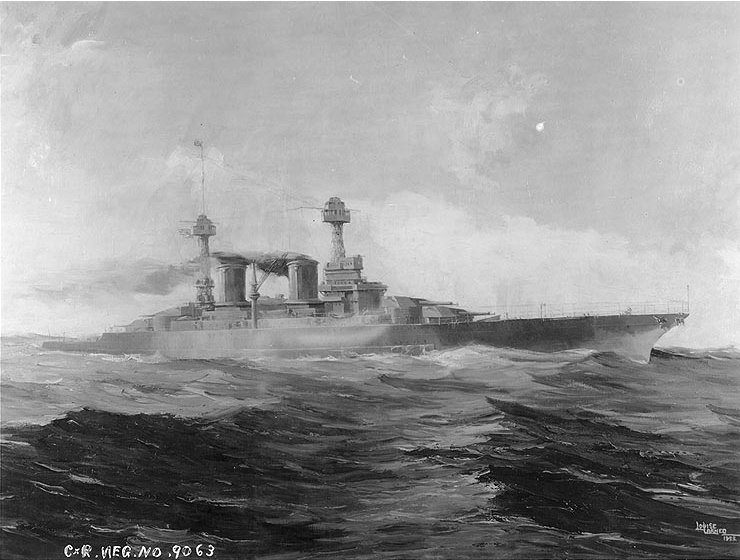
\includegraphics[scale=0.5]{Glava7/x1T2QXuUh1k.jpg}
	%	\label{fig:scipion} % Unique label used for referencing the figure in-text\end{document}
	%	%\addcontentsline{toc}{figure}{Figure \ref{fig:placeholder}} % Uncomment to add the figure to the table of contents%----------------------------------------------------------------------------------------
	\caption{Так должны были выглядеть линейные крейсера типа Лексингтон}%	CHAPTER 2
\end{figure}

В целом японские проекты судов как минимум не уступали по ТТХ американским, а кое-в-чём и превосходили их. Далеко не факт, что в конкурентной борьбе Япония сумела бы встать вровень с парой ведущих морских сил планеты, но Соглашение жестко и недвусмысленно задавало Императорскому флоту его потолок. Его будущее должно было быть похоронено ещё на стапеле, как и существенная часть его прошлых достижений. Стоит помнить и об относительности финансовых возможностей: каждый уже построенный линкор обошёлся для Японии куда дороже, чем для американцев или англичан, если брать не абсолютные величины, а доли от бюджета и доходов, так что их списание было тем более болезненным.

Видя непреклонную волю США и Британии и готовность Франции и Италии подписать Соглашение, японцы попытались хотя бы до конца торговаться. Япония настаивала на соотношении 5:5:3,5 и добивалась права достроить линкор «Муцу» типа «Нагато».

\begin{figure}[h!tb] 
	\centering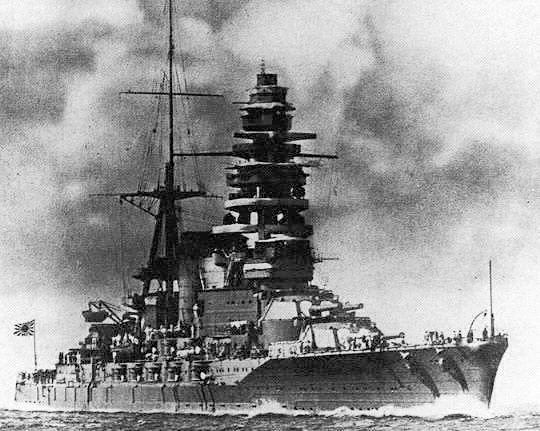
\includegraphics[scale=0.5]{Glava7/DRipb4WQs_c.jpg}
	%	\label{fig:scipion} % Unique label used for referencing the figure in-text\end{document}
	%	%\addcontentsline{toc}{figure}{Figure \ref{fig:placeholder}} % Uncomment to add the figure to the table of contents%----------------------------------------------------------------------------------------
	\caption{Линкор Муцу}%	CHAPTER 2
\end{figure}

 В результате длительной дискуссии, которую нет смысла здесь пересказывать, стороны пришли к следующему: Япония получила право достроить линкор Муцу, США — два линкора - «Колорадо» и «Вест Вирджинию», Британия — построить два новых линкора — «Нельсон» и «Родней» с учётом ограничений по водоизмещению и калибру орудий. Взамен Япония дополнительно утилизировала 1 корабль, США — 2, а Британия по вступлении в строй новых кораблей — 4. Соотношение тоннажей 5:5:3 (или 3:3:1,75) осталось без изменения. Взамен, немного подсластив пилюлю, США и Англия согласились ограничить строительство и укрепление военных баз на островах Тихого океана.

Но самое худшее ждало Японию впереди. Договор девяти держав от 6 февраля 1922 года, подписанный всеми участниками Конференции – её итоговый документ. Бумага эта, воплотившая в себе все худшие японские опасения, сама по себе весьма интересна. Титульно Договор касался обеспечения гарантий территориальной целостности Китая и уважения его суверенитета. При этом прописывавшийся в Договоре запрет на получение одной из держав-подписантов специальных прав и привилегий, которые могут нанести ущерб правам и интересам иных государств-участников договора в действительности был ничем иным, как ограничением китайского суверенитета – ведь и Поднебесная фактически лишалась права оказывать предпочтение тому или иному из своих партнёров. Сложно сказать, приходила ли подобная мысль американским авторам документа и, если да, сразу ли они решили её проигнорировать. Как бы там ни было, Договор в полной мере реализовывал именно концепцию Соединённых Штатов по китайскому вопросу: провозглашался принцип «открытых дверей и равных возможностей» по отношению к Китаю в области торговой и предпринимательской деятельности, любые формальные и неформальные зоны преимущественных интересов, экономических и, тем более, военно-политических, устранялись. Только чистая конкуренция. Кому это было выгодно? Назову лишь несколько достаточно красноречивых цифр. Имея в 1920 году всего 6\% мирового населения, США сосредоточили в своих руках 66\% мировой добычи нефти, 60\% меди, 60\% алюминия, 50\% угля, 20\% добычи золота, 85\% производства автомобилей. Одновременно с Договором девяти держав 6 февраля 1922 года был подписан Трактат о китайском таможенном тарифе, где формально закреплялось таможенное неравноправие Китая, положение, при котором Поднебесная окончательно делалась объектом коллективной эксплуатации держав.

За день до Договора, 5 февраля 1922 года, Япония вынуждена была подписать отдельное китайско-японское соглашение об эвакуации японских войск из китайской провинции Шаньдун, а также о возвращении Китаю железной дороги Циндао — Цзинань и территории Цзяо-Чжоу. Иными словами, были ни много ни мало пересмотрены положения Версальского договора. Параллельно глава японской делегации дал обязательство, что японское правительство не будет требовать от китайского правительства выполнения пятой группы «двадцати одного требования» Японии о назначении японских советников при китайском правительстве, фактически и так не принятой китайцами. На практике это была скорее индульгенция на то, чтобы игнорировать и остальные 16 принятых пунктов.

Единственное требование Китая, которое Япония отклонила, было требование о выводе японских войск из Южной Маньчжурии – из взятых с боем Порт-Артура и Дальнего. Может быть, причина была в том, что адмирал Томосабуро сам воевал в Русско-японскую, может осознание того, что подобного масштаба унижение может привести к немедленному социальному взрыву в стране. Но всё равно это был полный позор и полное поражение. Япония потеряла всё. Помимо всего описанного выше в отношении Китая, закреплённого документально, очевидно, были достигнуты и договорённости по уходу японских войск с русской территории. С весны 1922 начинается процесс быстрого свёртывания экспедиционных сил. Последний японский солдат покинет Владивосток 25 октября 1922 года. Единственное, что выгадала Япония от своего участия в Интервенции – вывезенные материальные ценности и переданная им на хранение белыми часть царского злотого запаса. У меня нет точных цифр, которые позволяли бы судить о том, отбили эти ценности расходы, или нет, но говорить о большой прибыли точно не приходится. Ну а 15 ноября 1922 – менее чем через месяц после ухода японцев, проект ДВР был зарыт, республика была ликвидирована и включена напрямую в состав РСФСР. Комбинация советского правительства окончилась блистательным успехом.

Все беды, просыпавшиеся, как град, на голову Японии, кажется, перечислены – осталось ответить на один, но принципиальный вопрос: почему японцы согласились на всё это? Лучше всего отразить причины уступчивости Империи Восходящего солнца можно тремя словами: неожиданность, неспособность, изоляция.

Выше уже говорилось о том, что, хотя в принципе от Конференции ничего хорошего не ожидалось, никто и подумать не мог, что Японию будут нагибать так грубо и отбирать у неё так много. Руководство империи было готово на торг, на какие-то локальные уступки, которые потом, может даже, и исполнять на самом деле не придётся, на продолжение (а инерционный сценарий всегда воспринимается как более естественный) той политики, которая имела место в 1914-1919. Вместо этого состоялся прямой пересмотр положений Версальского договора по вопросу Шаньдуня, да и вообще на Вашингтонской конференция Япония фактически оказалась в положении Германии на Парижской. Нет, конечно, она, в отличие от немцев в 1919, имела право голоса – вот только это был глас вопиющего в пустыне. Китай – очевидный враг, США и Британия со всеми 5 её доминионами договорились заранее и тоже заняли антияпонскую позицию, для Франции, Италии, Бельгии и Португалии Дальний Восток был второстепенным направлением, но вот отношения с США были очень важны и никто не желал портить их из-за японцев. Для Нидерландов, конечно, были более чем значимы их обширные владения, ныне ставшие Индонезией, но слабеющее королевство боялось (как покажет ВМВ – обоснованно) того, что Япония, гораздо более сильная и проводящая активную политику экспансии рано или поздно обратит внимание и на южные моря – и тогда голландцам будет нечего ей противопоставить. Сочетание предельно жестких требований и того, что у всех остальных, кроме японцев, они не вызывали возражений создало просто ошеломляющий эффект. Тем более – вспоминаем о неспособности – на Конференции Империю Восходящего солнца представляли отнюдь не лучшие её дипломаты и вообще умы. Крайне несвоевременное убийство премьера Такаси также сыграло свою роль – Токио и оставшиеся там руководители тоже едва ли могли помочь делегации в Вашингтоне, особенно на начальном этапе Конференции.

Япония не могла оказать влияния на ход Конференции, на круг рассматриваемый проблем и тон их обсуждения. Единственное, что можно было сделать – это под конец демонстративно хлопнуть дверью. Но это – пощёчина всем оставшимся, противопоставление себя им, изоляция, ярлык агрессора. Наконец, Соединённые Штаты в этом случае могли бы принять вполне реальные и весомые меры. Конечно, едва ли можно было ожидать линкоров ВМС США в заливе Суруга и в гавани Токио, тем более – десанта на территории империи. Но это было и ни к чему. Американцы и китайцы могли просто вдруг “позабыть” о 16 пунктах, принять любые решения на Конференции уже без японцев – а в случае их ухода антияпонскую природу её, задачу сдерживания Японии можно бы было уже не скрывать, а после перебросить мяч на японскую половину поля. Играйте! Действуйте! Попытаетесь давить на Китай силой – получите спонсирование и поддержку деньгами и оружием самых радикальных антияпонских сил, которые там удастся найти. Предпримите прямую агрессию – получите жесткий ответ в области экономики с перспективой полной изоляции не только дипломатической, но и торговой. Эмбарго на стратегические виды сырья, давление на корпорации, готовые сотрудничать с Империей Восходящего солнца буквально в любых отраслях. А что такое для Японии с её экономической структурой изоляция, думаю, напоминать вновь не нужно. И самураям останется только два варианта – либо договариваться, либо самим бросаться лбом на американскую стенку. Очень похоже в итоге все и получится, только 20 лет спустя...

Япония приняла все условия. Но не смирилась с ними. Психологически в японском обществе вызрело то же, что и в Германии и Италии, но только даже в большем масштабе – ощущение того, что с ними обошлись несправедливо, что при первой возможности нужно что-то с этим сделать, нужно переиграть. У немцев была теория “ножа в спину” и всё погубившей революции, но, в общем то, все понимали, что к осени 1918 Германская Империя так и так проигрывала войну – разве только условия мира могли бы, всё же, оказаться несколько более мягкими. У итальянцев был комплекс недооценённости их роли в ПВМ, чувство, что им недодали. На нём весьма умело сыграет будущий дуче Бенито. Но и там все холодные головы понимали – объективно Италия воевала плохо и своими силами не сумела захватить даже и того, что в итоге приобрела волей союзников. Помнили и битву при Капоретто, и то, какие экономические трудности пережила страна. Идея награды не по успехам, а по потерям и страданиям – она приятная, но так в международной политике это не работает. А вот Япония никого и ни о чём не просила, добилась всего сама, причём после череды военных побед – вспомним, что и Японо-китайская, и Русско-японская, и участие Японии в ПМВ – всё это победы империи. И всё это у неё отобрали. Просто из ревности и жадности. Просто потому, что обладали для этого достаточной силой. С 1922 года идея о необходимости непрерывного военного усиления, постоянной готовности, становится в Японии всеобщей. Упавшее было после Рисовых бунтов влияние военных начинает неуклонно возрастать. Вообще Вашингтонская конференция оказалась ещё и страшным ударом по японскому парламентаризму и демократии. Во главе страны в момент подписания всех постыдных документов и договоров было партийное, гражданское правительство. Конечно же, все беды приписали его слабости. Если в начале ноября 1921 только такие как Коничи Накаока верили в то, что люди вроде покойного Такаси – негодяи и предатели, то теперь большинство было убеждено: наверху засела клика едва ли не изменников, отстаивающих узкопартийные интересы и связанных с парой тройкой финансово-промышленных групп, которые в обмен на сохранение торговых контактов с США предали и продали достижения нации. При этом, не будь Рисовых бунтов, останься у власти кто-то вроде маршала Тэраути Масатаке, далеко не факт, что по зрелом размышлении не пришлось бы примириться с решениями конференции и им.

Тем не менее, после 1922 года все попытки выстроить партию – не некий официозно-чиновный орган, работа которого только в том, чтобы призывать сплотиться вокруг священной персоны императора, а именно партию со свой программой и нормальными кадрами, которая устраивала бы и народ и находящихся у кормила власти, могла бы служить связующим звеном между ними, провалились с треском. Резко усиливаются – и в верхах и в низах те, кто вообще не настроен на какой-либо компромисс. С одной стороны 15 июля 1922 года создаётся и начинает весьма активно и успешно действовать Коммунистическая партия Японии, а чуть позже после Марша на Рим 27-30 октября 1922 и прихода мировой известности итальянскому фашизму резко усиливаются крайне правые. С другой большой пласт чиновничества и, особенно, генералитета, начинает считать в принципе опасными все эти “игры в демократию”. Благо 29 ноября 1921 года достигший совершеннолетия наследник престола – Хирохито становится регентом при недееспособном отце. У страны вот-вот может появиться полноценный император.

Но это, всё же, пока дело будущего. А пока вскоре после возвращения из Вашингтона адмирал Като Томосабуро был назначен премьер-министром. 

\begin{figure}[h!tb] 
	\centering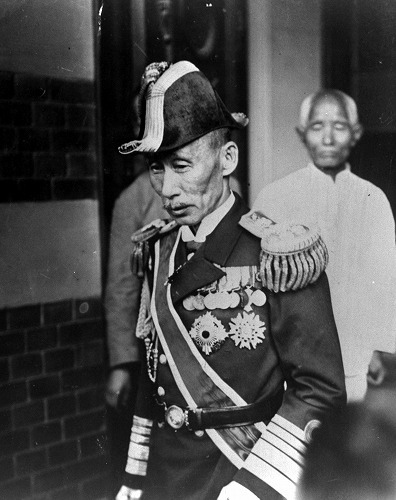
\includegraphics[scale=0.5]{Glava7/DWql6zvETIs.jpg}
	%	\label{fig:scipion} % Unique label used for referencing the figure in-text\end{document}
	%	%\addcontentsline{toc}{figure}{Figure \ref{fig:placeholder}} % Uncomment to add the figure to the table of contents%----------------------------------------------------------------------------------------
	\caption{Адмирал Томосабуро в бытность премьер-министром}%	CHAPTER 2
\end{figure}

Собранный им кабинет состоял преимущественно из членов Палаты Пэров парламента, непопулярных в армейской среде. Его деятельность в 1922—1923 годах была связана главным образом с реализацией подписанных в Вашингтоне соглашений, а именно разделкой недостроенных военных кораблей, выводом японских войск с Шаньдунского полуострова и из Советской России. Сам факт того, что пришлось собирать кабинет, практически полностью исходя из задачи исполнения условий того, что было подписано в Вашингтоне, очень показателен: японцы по настоянию и под надзором внешних сил были вынуждены делать то, что считали для себя прямо невыгодным и, что ещё хуже, постыдным. В значительной мере даже по форме это смотрелось как капитуляция. Капитуляция в войне, которую Япония не проигрывала. Капитуляция угрозам и бумагам. В том числе и отсюда несговорчивость даже в самых жестких условиях будущих японских правительств.

Здесь уместно более подробно поговорить о кораблях и их судьбе. Первенец японского дредноутного флота – линкор Кавати до 1922 не дожил: 12 июля 1918 года, когда «Кавати» стоял на якоре в заливе Токуяма, в пороховом погребе взорвался кордит. Корабль затонул, погиб 621 человек из 1 059, находившихся на борту. Впоследствии Кавати был поднят со дна и разобран на металл. А вот его собрат Сэтцу пал жертвой именно Вашингтонской конференции. В 1922 году на верфи Курэ с Сэтцу сняли вооружение. В 1924 году линкор был выведен из состава флота и превращен в хорошо бронированный корабль-мишень. Вообще старый дредноут ждала довольно любопытная судьба - в 1937—38 на Сэтцу установлено дистанционное управление по радио; кораблем-мишенью управляли с пульта на эсминце «Юкадзэ». Но тип Кавати так и так был устаревшим. Когда же речь шла о более сильных судах, японцы хитрили на грани фола. Так, согласно Вашингтонскому соглашению, должны были быть ликвидированы как боевые суда два из четырёх линейных крейсеров типа Конго. Японцы во-первых сверх всякой меры затягивали процесс их вывода из состава линейного флота – так линейный крейсер Хиэй был выведен и преобразован в учебный артиллерийский корабль (снятие части котлов, брони, вооружения) только в 1929 году. Предлоги были самые разные вплоть до откровенно смехотворных – оказывается, в течение 7 лет Япония не могла найти верфь, которая могла бы заняться Хиэй, из-за постоянных забастовок рабочих! Во-вторых, что куда серьёзнее и, по большому счёту, не имело прецедентов – это возможность расконсервации и модернизации вроде бы как списанных кораблей. Во многом именно эту возможность, судя по всему, должен был проработать и реализовать адмирал Томосабуро. И Хиэй и его систершип Харуна были перед Второй мировой, уже после окончания действия Соглашения (1936 год), вновь введены в строй. Дредноуты Фусо и Ямасиро, Исэ и Хюга, а также Нагато, имевшиеся к дате подписания 6 февраля 1922 в составе Императорского флота Японии, так в нём и остались. К ним добавился оговоренный в тексте документа систершип Нагато – линкор Муцу. Остальные же находившиеся ещё не в полностью готовом к роковому сроку корабли ждала иная судьба.

В первую очередь после Вашингтонского соглашения японцы отменили постройку ещё не заложенных, но уже заказанных линкоров типа Кии, которые должны были быть построены в количестве четырёх штук. Формально постройка не получивших названия линкоров № 11 и № 12 была отменена 19 ноября 1923 года, а 14 апреля 1924 — головного Кии и Овари. Сложнее было с парой дредноутов типа Тоса – Тоса и Кага. 

\begin{figure}[h!tb] 
	\centering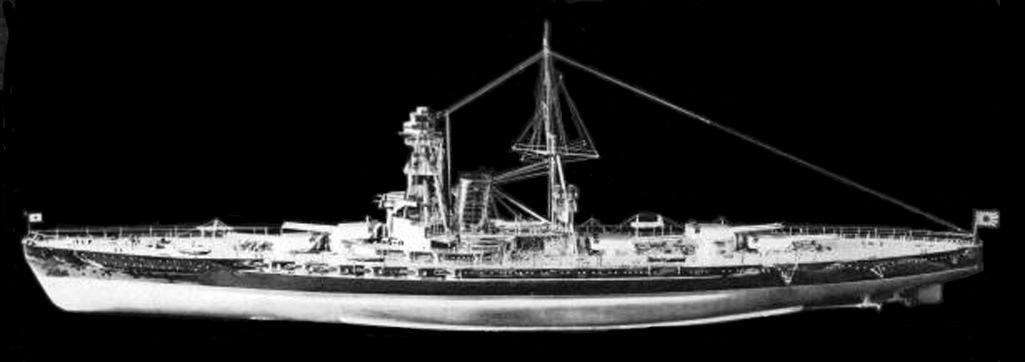
\includegraphics[scale=0.3]{Glava7/MIoBH1FflI8.jpg}
	%	\label{fig:scipion} % Unique label used for referencing the figure in-text\end{document}
	%	%\addcontentsline{toc}{figure}{Figure \ref{fig:placeholder}} % Uncomment to add the figure to the table of contents%----------------------------------------------------------------------------------------
	\caption{Так должны были выглядеть готовые линкоры типа Тоса}%	CHAPTER 2
\end{figure}

Оба были уже в весьма высокой степени готовности. Собственно, спуск на воду Тоса ожидался в октябре 1921 – ещё до начала Конференции, но вот здесь действительно подвели забастовки работников верфи Кобэ. Особым пунктом Соглашения оговаривалась возможность для держав достроить два ранее заложенных линкора в качестве авианосцев, не обращая внимания на предельный тоннаж для последних в 21 000 тонн. Но японцы предполагали воспользоваться этим правом в отношении двух линейных крейсеров серии Амаги – о них чуть ниже. Это значило, что Тоса и Кага обречены. В случае с головным кораблём все вышло так: 5 мая 1922 года, в соответствии с подписанным соглашением, строительство линкоров «Тоса» и «Кага» было отменено. В августе 1922 года недостроенный «Тоса» был перемещен в Куре. Пятьдесят тысяч человек наблюдали, как линкор буксировался из гавани пятью буксирами. 

\begin{figure}[h!tb] 
	\centering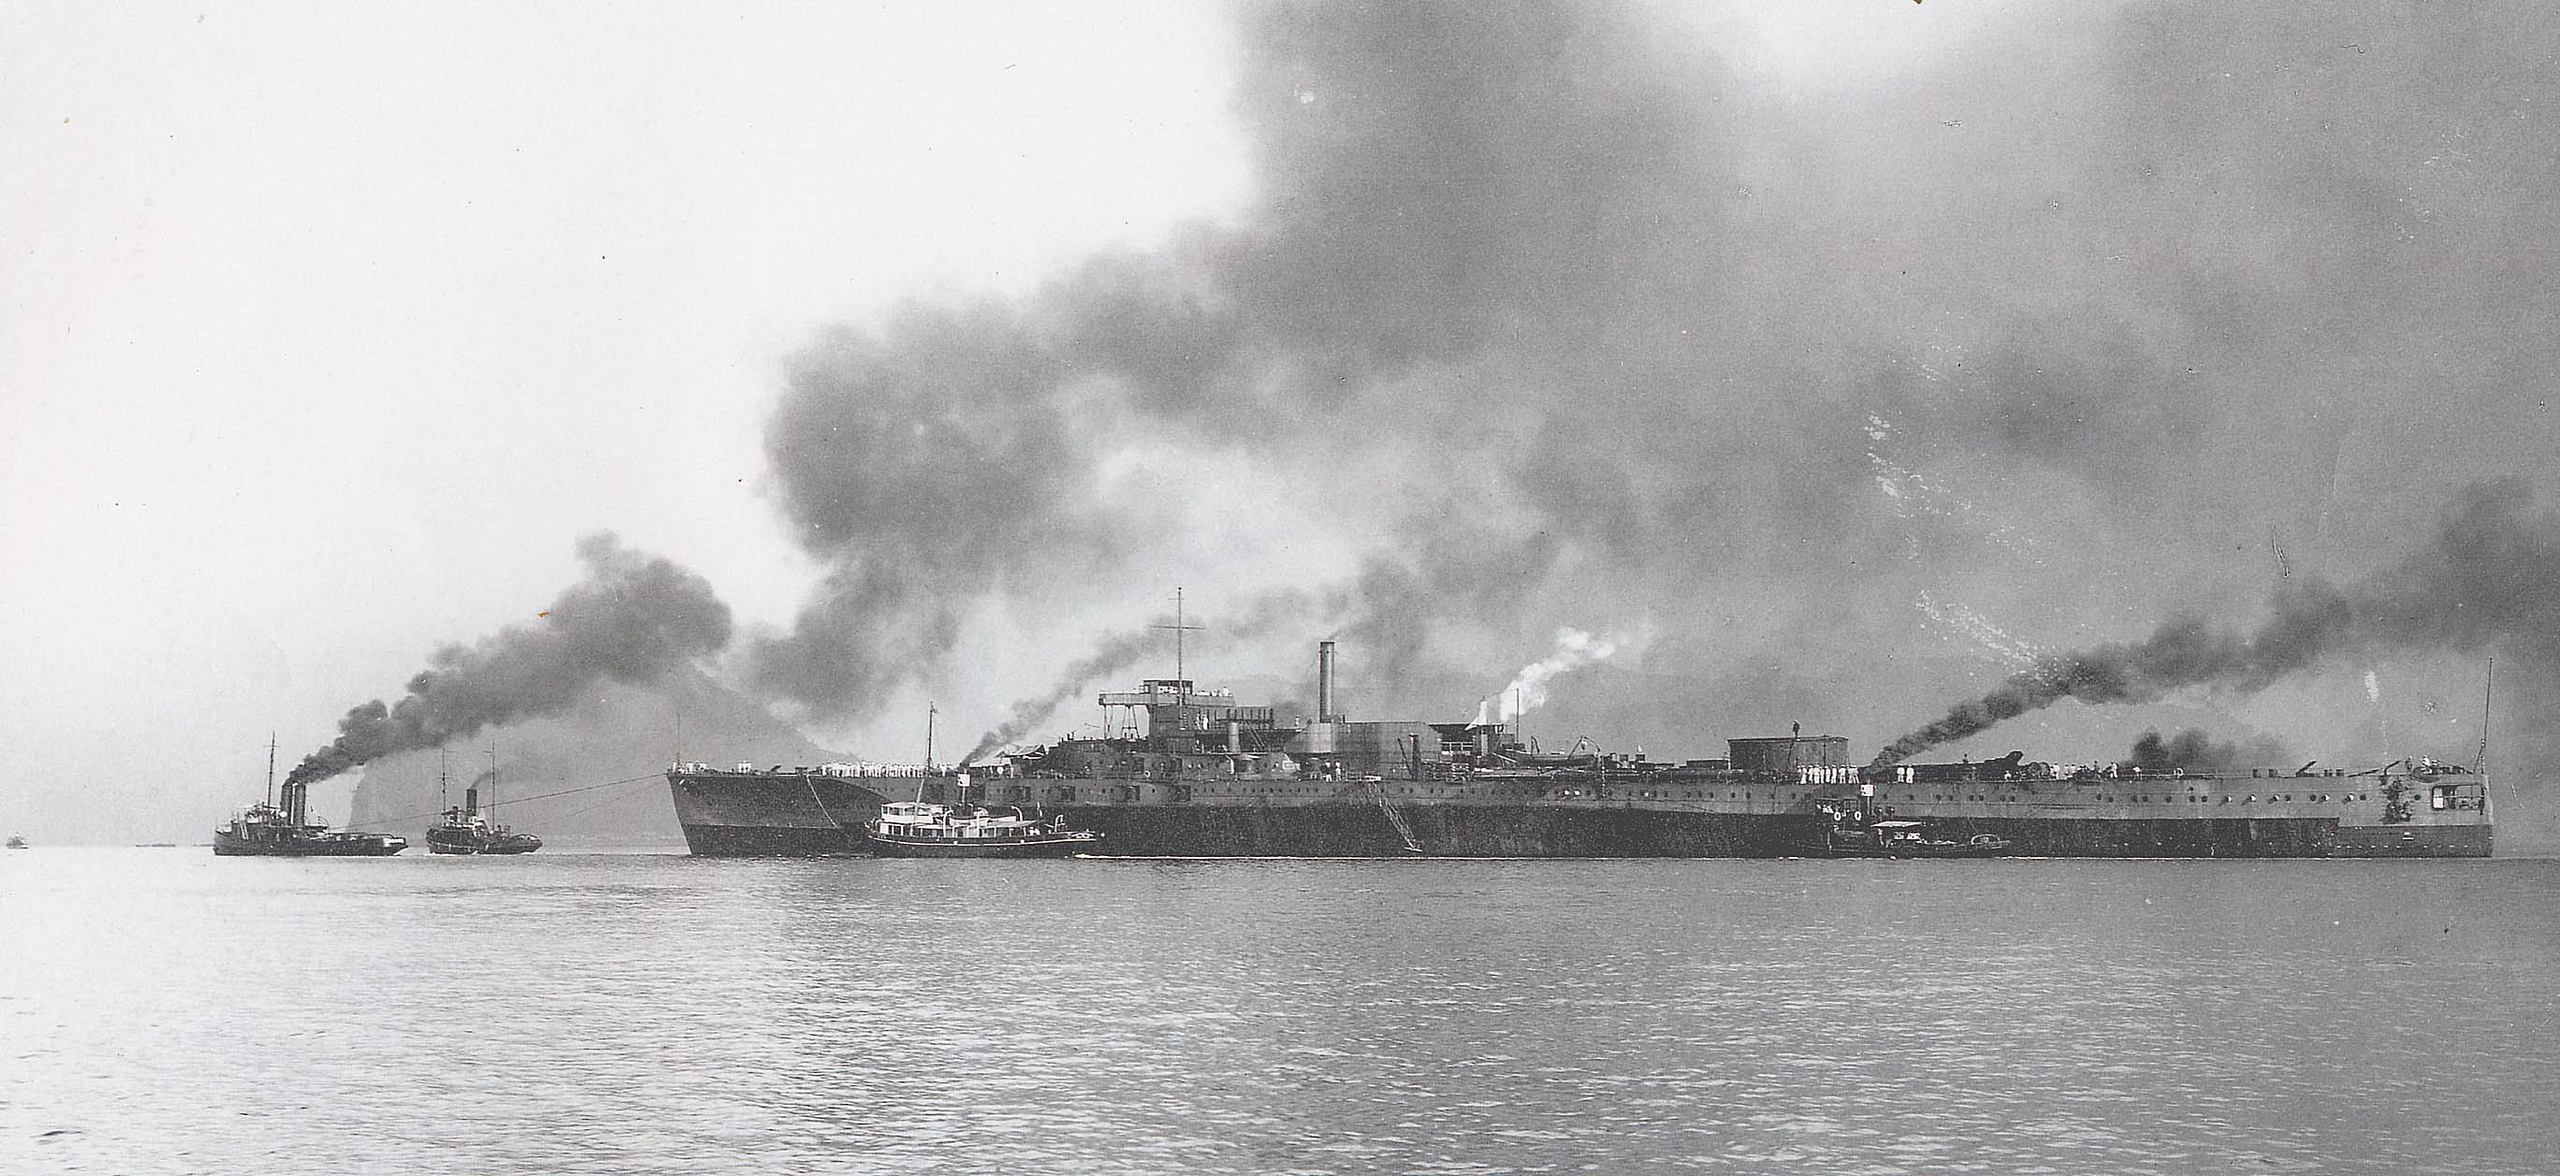
\includegraphics[scale=0.2]{Glava7/6xIYCX30oEs.jpg}
	%	\label{fig:scipion} % Unique label used for referencing the figure in-text\end{document}
	%	%\addcontentsline{toc}{figure}{Figure \ref{fig:placeholder}} % Uncomment to add the figure to the table of contents%----------------------------------------------------------------------------------------
	\caption{Буксировка недостроенного дредноута Тоса}%	CHAPTER 2
\end{figure}

К тому времени на линкоре были смонтированы барбеты для 406-миллиметровых орудий, но башни и орудия не были установлены, а отверстия в главной палубе были покрыты металлическими листами. Корпус корабля — палуба и надстройки были закончены, так же были смонтированы — мостик, боевая рубка, мачта светового сигнала в кормовой части второго барбета. Боевая рубка была снабжена оборудованием моста управления, поскольку для этого не было другого подходящего места. Тоса оставался в Куре до середины 1924 года. 1 апреля 1924 года, корпус недостроенного линкора был подготовлен к испытаниям и передан военно-морскому флоту для использования в качестве корабля мишени – так недостроенный дредноут служил флоту ещё несколько месяцев.

14 января 1925 года, Морское министерство Японии отдало приказ уничтожить линкор в течение одного месяца. Главнокомандующий военно-морским районом Куре, предписал к 1 февраля закончить приготовления и до 10 февраля затопить линкор. Для этого тоже уже обречённый линкор Сэтцу, упоминавшийся выше, должен был отбуксировать Тосу на расстояние 16 километров к западу от острова Окиносима к месту затопления. Но линкор словно не желал так бесславно отправляться на дно. 3 февраля Тоса перевели из Куре в залив Саики, откуда 6 февраля вывели на буксире, намереваясь привести его к месту затопления, но помешал сильный шторм и корабли вернулись. Вторая попытка была предпринята 8 февраля в 10:00. В машинное отделение линкора были загружены взрывные заряды — два контейнера по 30 килограмм взрывчатки в каждом, в двойном дне разместили два 356 мм снаряда. Заряды должны были взорвать, используя электрические плавкие предохранители. Восьмого февраля при подрыве заряды не сработали. После этой неудачи девятого числа на борт «Тоса» была отправлена команда для затопления корабля. В 01:25 в машинном отделении «Тоса» открыли шесть кингстонов. Вскоре после этого «Тоса» стал крениться на правый борт и медленно погружаться кормой в воду. В 03:50 крен увеличился, и судно скрылось с поверхности воды в 07:00.

А вот Кага ждала совершенно другая судьба – его всё же достроили в качестве авианосца и базировавшиеся на его борту самолёты поучаствовали в ударе по Перл-Харбору. Как так вышло? Как было сказано выше, к переделке готовили корабли типа Амаги. Четвёрка линейных крейсеров из которых Амаги и Акаги были заложены в 1920 году и имели готовность порядка 40\%, а Атаго и Такао – в 1921 и имели более низкую степень готовности должны была кончить по-разному. Вторые два линейных крейсера разобрали прямо на стапеле. Первые два начали переделывать. Акаги будет спущен в новом качестве 22 апреля 1925 года, став первым тяжёлым авианосцем ВМФ Японии. До своей модернизации 1934-1938 это был весьма экзотический корабль. Акаги стал первым опытом строительства крупных авианосцев в Японии, поэтому многие элементы отрабатывались на нём впервые. Сказалось также и изначальное происхождение корабля как линейного крейсера. Самым необычным элементом являлось наличие сразу трёх (реально двух) полётных палуб. 


\begin{figure}[h!tb] 
	\centering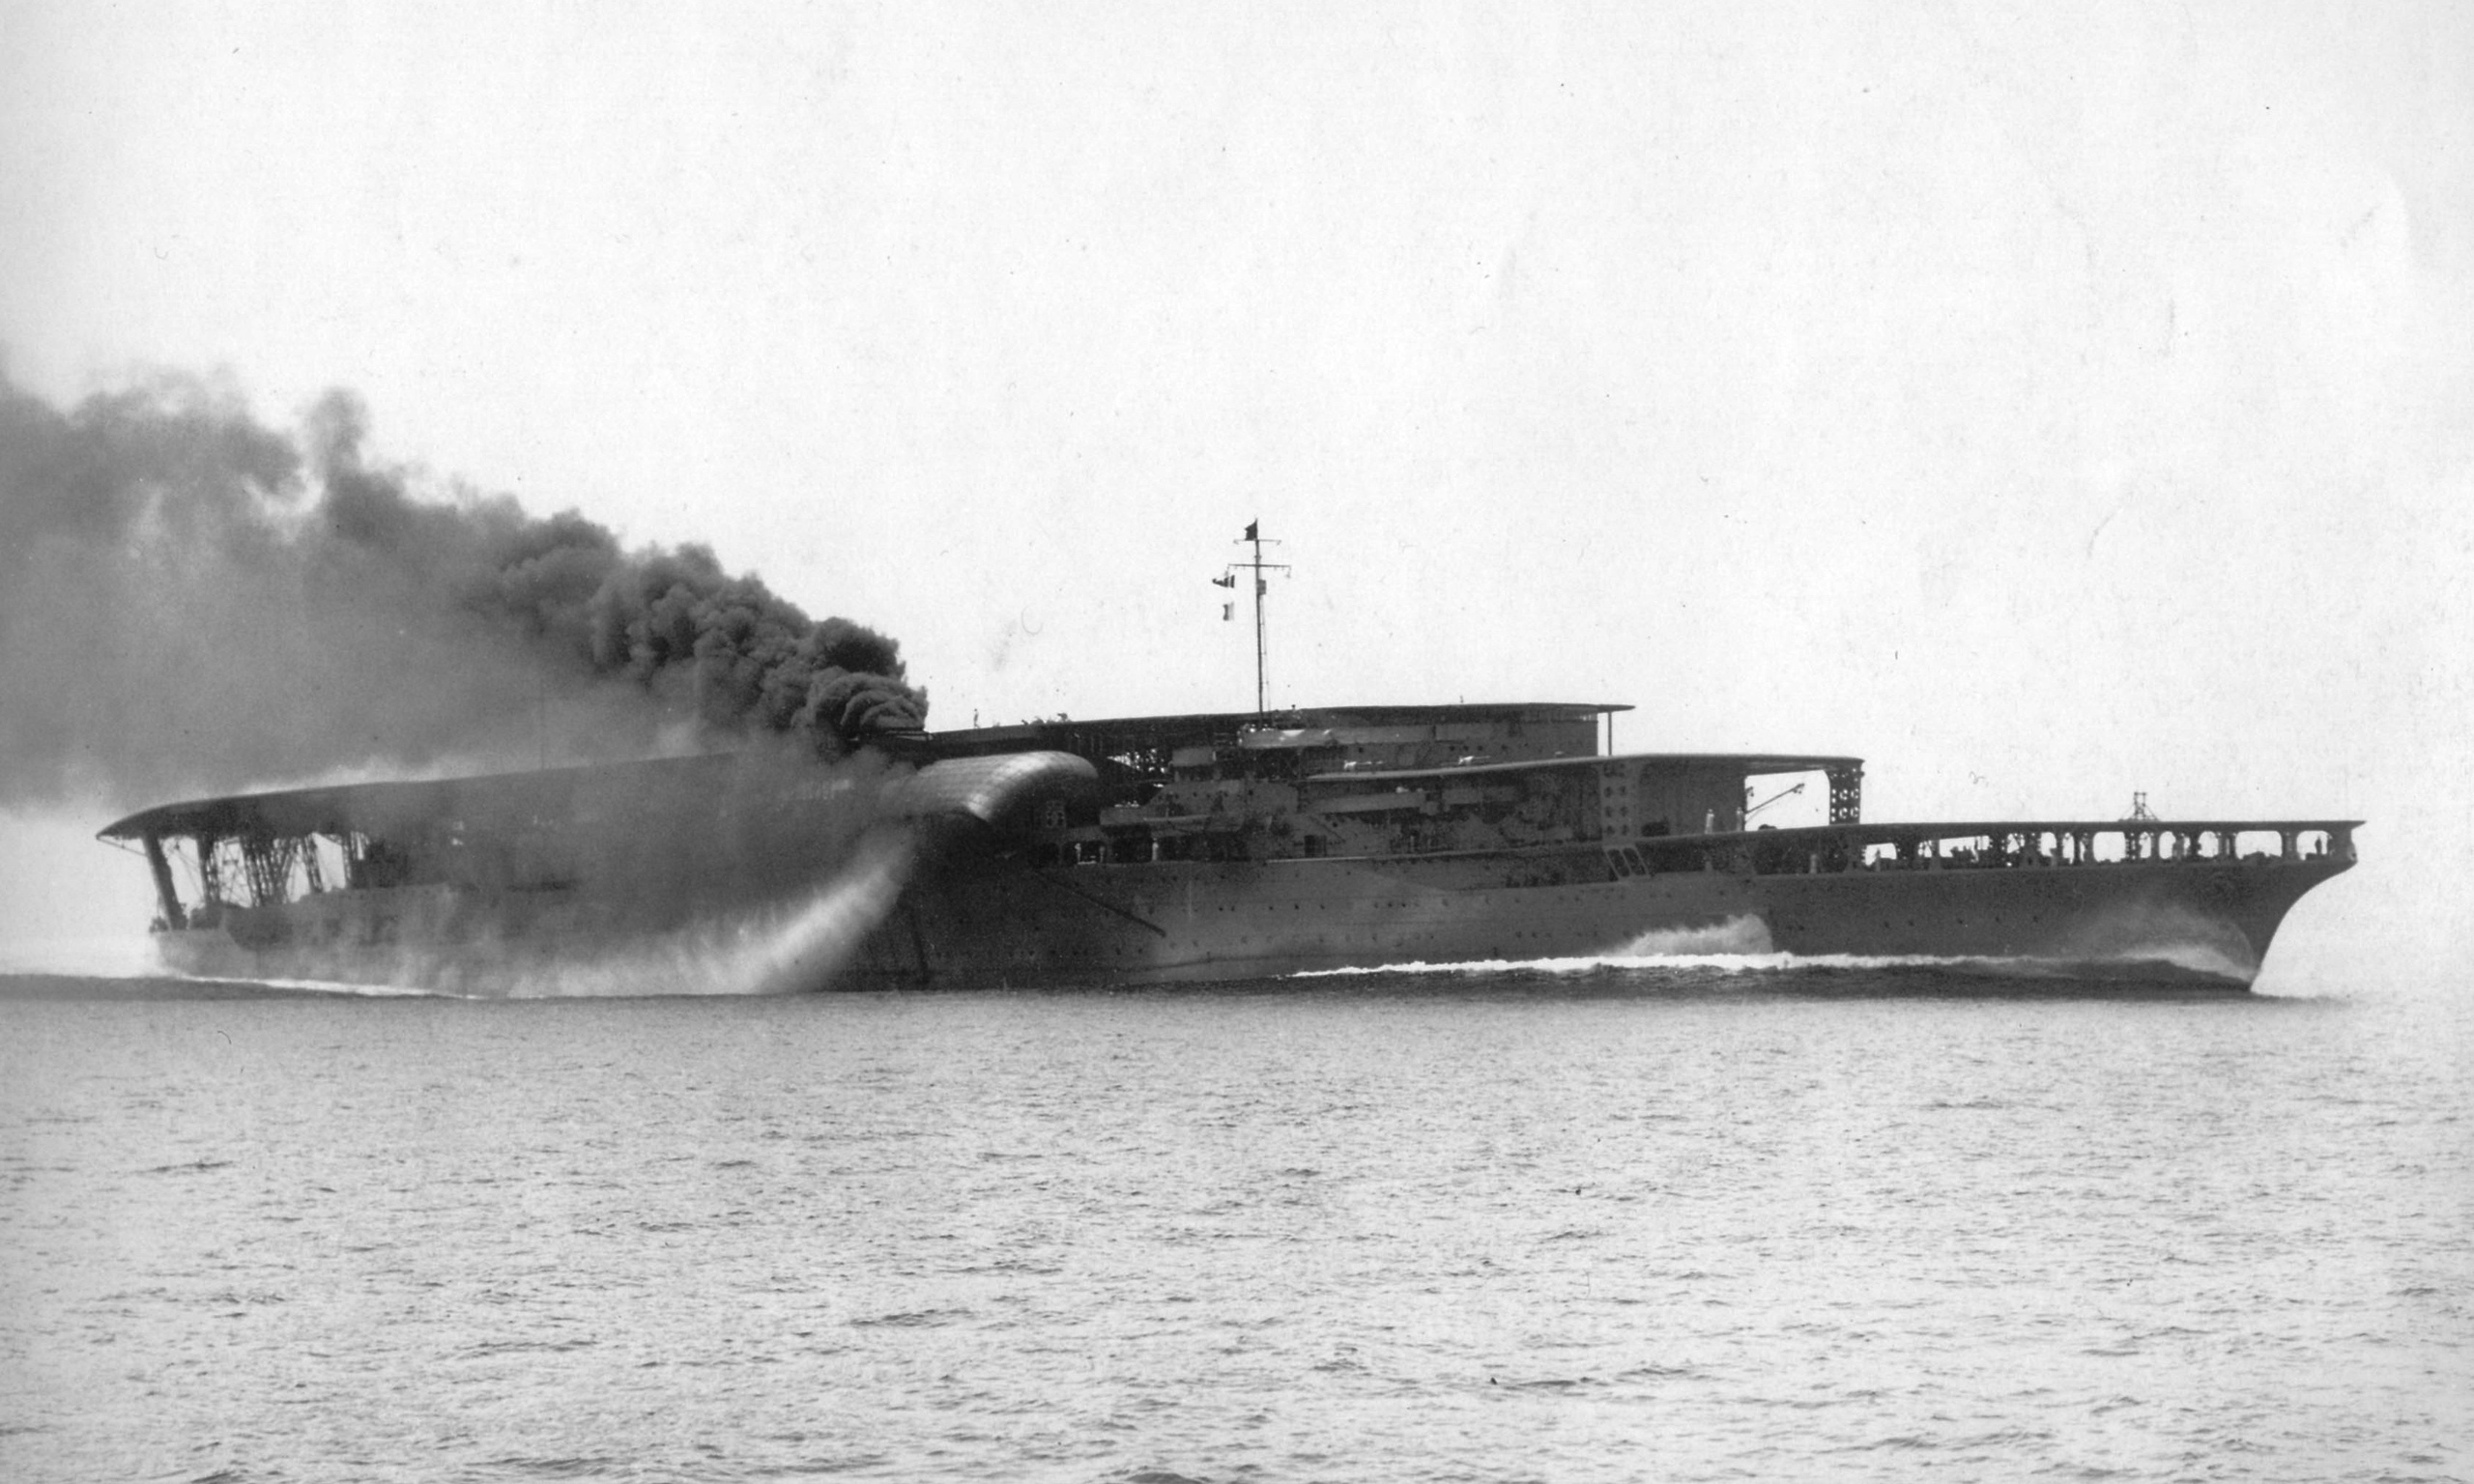
\includegraphics[scale=0.2]{Glava7/esXdRV6ZeqQ.jpg}
	%	\label{fig:scipion} % Unique label used for referencing the figure in-text\end{document}
	%	%\addcontentsline{toc}{figure}{Figure \ref{fig:placeholder}} % Uncomment to add the figure to the table of contents%----------------------------------------------------------------------------------------
	\caption{Акаги до модернизации}%	CHAPTER 2
\end{figure}

Верхняя полётная палуба длиной 190 метров и максимальной шириной 30,5 метров предназначалась для взлёта и посадки самолётов. Средняя палуба начиналась в районе мостика и была длиной всего 15 метров, а ширина была сильно ограничена орудийными башнями. Нижняя полётная палуба длиной 55 метров и максимальной шириной 23 метра предназначалась для старта торпедоносцев. Наличие трёх палуб должно было облегчить экипажу обслуживание самолетов и обеспечить старт максимально возможного количества самолётов за ограниченное время. Акаги был авианосцем, способным одновременно выпускать и принимать самолёты. Расположение полётных палуб позволяло организовать непрерывный цикл. После старта и выполнения задания самолёт приземлялся на главную полётную палубу, его опускали в ангар, заправляли, вооружали и самолет снова отправлялся в бой с передней палубы. При этом ни на одной из совершенно гладких палуб не было “острова” управления. Серьёзным недостатком авианосца было и отсутствие у ангаров стен, которые установили лишь в дальнейшем после того, как произошло несколько аварий из-за захлестывания ангаров водой.

А вот Амаги так никогда и не переоборудовали. Дело в том, что судьба ещё не окончила тешиться над Страной Восходящего солнца. Она подготовила для неё, всё же, пожалуй, самую страшную катастрофу – природную. 1 сентября 1923 года произошло так называемое Великое землетрясение Канто. Одно из самых сильных в истории Японии. И первое – по числу жертв и масштабу разрушений. Тяжёлые повреждения получил и Амаги – настолько, что, в конечном счете, его сочли целесообразным разобрать, отдав предпочтение переделке в авианосец Каги типа Тоса.

Но, конечно, Амаги потери страны не ограничились. Подземные толчки (магнитуда 8,3 балла) практически под ноль разнесли важнейшие города страны – Йокогаму и столичный Токио. Собственно, эпицентр землетрясения и располагался в 90 км к юго-западу от Токио в море возле острова Осима в заливе Сагами. Всего за двое суток произошло 356 подземных толчков, из которых первые были наиболее сильными. В заливе Сагами из-за изменения положения морского дна поднялись 12-метровые волны цунами, которые опустошили прибрежные поселения. В Йокогаме, находившейся в 65 км от эпицентра, в результате подземных толчков было сразу же разрушено не менее пятой части зданий. Повсюду немедленно начались пожары, из-за сильного ветра огонь быстро распространялся. В порту горел разлившийся по воде бензин, пламя достигало 60 м в высоту. Большая часть противопожарных средств была уничтожена при первых же толчках, что серьёзно ограничило возможности по локализации пожаров. На железной дороге Токио — Йокогама с пути сошёл поезд, наткнувшись на вывороченные и скрученные рельсы.

\begin{figure}[h!tb] 
	\centering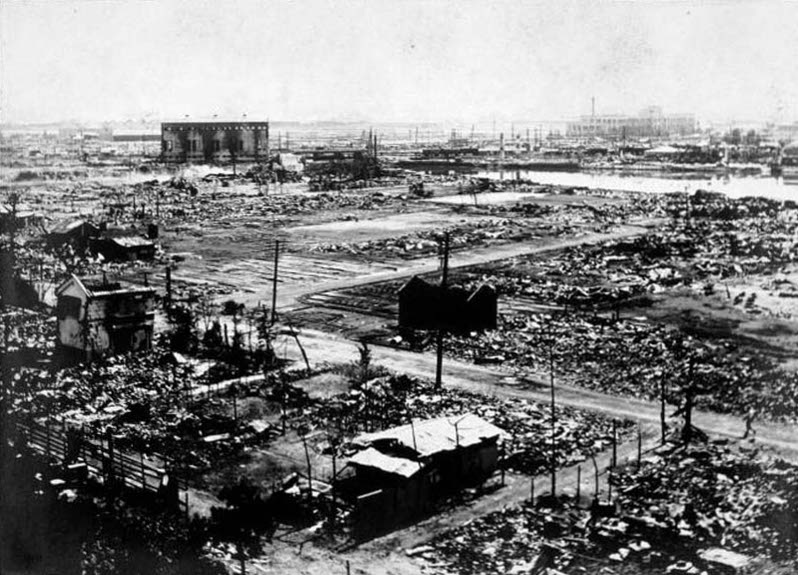
\includegraphics[scale=0.4]{Glava7/wXqFmTQB9Ms.jpg}
	%	\label{fig:scipion} % Unique label used for referencing the figure in-text\end{document}
	%	%\addcontentsline{toc}{figure}{Figure \ref{fig:placeholder}} % Uncomment to add the figure to the table of contents%----------------------------------------------------------------------------------------
	\caption{Последствия землетрясения в Йокогаме. Автору доводилось видеть эту фотографию, ошибочно иллюстрирующую последствия бомбардировки Хиросимы}%	CHAPTER 2
\end{figure}

В Токио, находившемся в 90 км от эпицентра, было разрушено меньше зданий, чем в Йокогаме (в процентном отношении), но также повсеместно начались пожары, разносимые сильным ветром, которые и причинили наибольший ущерб. Противопожарные средства уцелели, но землетрясение разрушило городской водопровод, во многих случаях пожарная техника не могла проехать по узким улицам. Спасаясь от подземных толчков и пожаров, жители бежали на открытые пространства — площади, парки, — но это не всегда помогало. На одной из площадей Токио погибло около 40 тыс. человек — они задохнулись, когда загорелись окружающие площадь дома. Всего же в стране число жертв согласно официальной статистике достигло 174 000 – уже огромная цифра, но много больше - 542 000 человек числились пропавшими без вести. Для сравнения в Первой мировой Япония потеряла убитыми 415 солдат. Вообще за два дня страна лишилась такого количества граждан, что совокупные потери убитыми Японо-китайской, Русско-Японской и Первой мировой можно было умножить на 10 – и всё равно они оказались бы меньше. Хотя страна и находилась в прямом смысле слова “на вулкане” всю свою историю, но такого ада не было никогда.

Помимо человеческих утрат громадными были и экономические потери. Материальный ущерб, понесённый Японией от землетрясения Канто, оценивается в 4,5 миллиарда долларов, что составляло на тот момент два годовых бюджета страны и в пять раз превышало расходы Японии в Русско-японской войне. Токио нужно было едва не заново строить. Только пожаром было уничтожено свыше 300 тысяч зданий (из примерно миллиона). В конечном итоге после землетрясения в столице сочли не подлежащими восстановлению около половины строений города. Из 675 мостов 360 было уничтожено огнём. Токио лишился всех каменных зданий. Устоял только отель «Империал», возведенный за год до этого знаменитым архитектором Фрэнком Ллойдом Райтом. Масштаб произошедшего в столице империи ясно виден по тому, что на полном серьёзе обсуждался вариант попросту бросить город, а столицу перенести. Причём в качестве одного из вариантов назывался Кэйдзё (ныне Сеул) – потому что там сейсмическая обстановка куда более стабильна.

Как назло буквально за несколько дней до землетрясения от рака толстой кишки на последней стадии скончался 24 августа 1923 года премьер Томосабуро, так что в итоге имел место ещё и кризис власти, многие принципиальные решения принимались несвоевременно и с запозданием. Вновь сделавшийся временным главой кабинета в самый худший момент из возможных несчастный дипломат Утида Косай передал 2 сентября власть в руки пожилого адмирала Ямамото Гомбэй – опытного и достаточно талантливого военного-управленца. С 1893 года Гомбэй исполнял обязанности заведующего хозяйством министерства флота, а с 1895 года — возглавлял военный отдел этого министерства. Во время первой японско-китайской войны он успешно руководил административными делами Шанхайской армии, за что был удостоен должности министра флота Японии. Был адмирал и в премьерском кресле с 20 февраля 1913 по 16 апреля 1914. Но, всё же, и Гомбэй явно был не вполне готов к той работе, которую ему пришлось выполнять после Великого землетрясения Канто.

Последствия бедствия общенационального масштаба буквально выбросили Японию из глобальной политики на несколько лет. Все средства, все ресурсы, вся воля и таланты управленцев должны были быть брошены на то, чтобы хоть как-то восстановить центральную часть страны. Колоссальное количество бездомных и безработных, рост бедности – ведь все обширные внешние проекты 1910-х, которые как раз в это время должны были бы принести первую серьёзную отдачу, не принесли ничего, кроме горького разочарования, сохраняющаяся атмосфера национального унижения – всё это способствовало тому, что внутриполитическая обстановка всё более накалялась. Борьба властей с оппозицией стала бескомпромиссной, жестокой, всё чаще – вооруженной. Компартию Японии не постеснялись обвинить в пожарах и беспорядках после землетрясения, против неё усилились репрессии, был убит председатель Комсомола Каваи Ёситаро. 23 декабря 1923 в ответ на репрессии против коммунистов (равно как и прочих социалистов и анархистов) член КПЯ, студент Дайсукэ Намба совершил неудачное покушение на наследного принца Хирохито. Тяжело переживавший это действительно прежде непредставимое для Японии деяние как персональный позор, ушёл в отставку, взяв на себя всю ответственность, премьер-министр адмирал Гомбэй. Следующий глава кабинета - Киёура Кэйго смог просидеть в кресле всего около полугода – с 7 января по 11 июня 1924, а потом тоже подал в отставку, не в силах справиться с нарастающим политическим кризисом.

Преемник - Като Такааки. Это имя нам уже встречалось прежде – именно в его бытность министром иностранных дел в кабинете Окумы Сигэнобу он принимал участие в составлении 21 требования. Но теперь совершенно иные времена. С 11 июня 1924 года по 28 января 1926 года Като Такааки возглавляет японское правительство наскоро сколоченной коалиции «трёх партий защиты Конституции» - т.е. всех тех, кто не желает радикальных перемен в жизни государства и общества. Однако перемены всё равно неизбежны. Параллельно готовится сразу два весьма важных новых закона. Первый – введение всеобщего избирательного права. Хотя, конечно, и с определёнными оговорками – ну и, разумеется, это не касалось женского пола. Итак, все подданные-мужчины старше 25 лет могли голосовать, если они жили не менее года в своем избирательном округе и не были бездомными. Таким образом, число избирателей увеличилось с 3,3 до 12,5 миллионов человек. А 22 апреля 1925 года был принят «Закон об охране общественного порядка», который предусматривает значительное ограничение свободы слова и собраний. В прессе его прозвали “закон об опасных мыслях”. Он предусматривал суровое наказание в 10 лет каторжных работ не только за любые антимонархические, антигосударственные действия, но и просто за “намерение” совершить их. Причём, разумеется, доказательства такого намерения могли трактоваться очень широко. Репрессии, направленные главным образом против демократических, рабочих организаций, обрушивались даже на неортодоксальные организации верующих, стремящихся к “обновлению мира”. Так, была разгромлена религиозная секта Омото-кё, отрицающая “божественный статус” императорской династии – это подвели под сомнения в законности ее правления. Лидеры организации были лишены свободы за “оскорбление трона”.

Но политические перемены не ограничились новым законодательством. В 1926 году 25 декабря скоропостижно и неожиданно в возрасте 47 лет скончался император Есихито. В жизни империи во всех смыслах – формальном и неформальном, начиналась новая эпоха – на трон уже не в статусе регента, а полновластно восходил император Хирохито с девизом правления Сёва, Просвещённый мир. 

\begin{figure}[h!tb] 
	\centering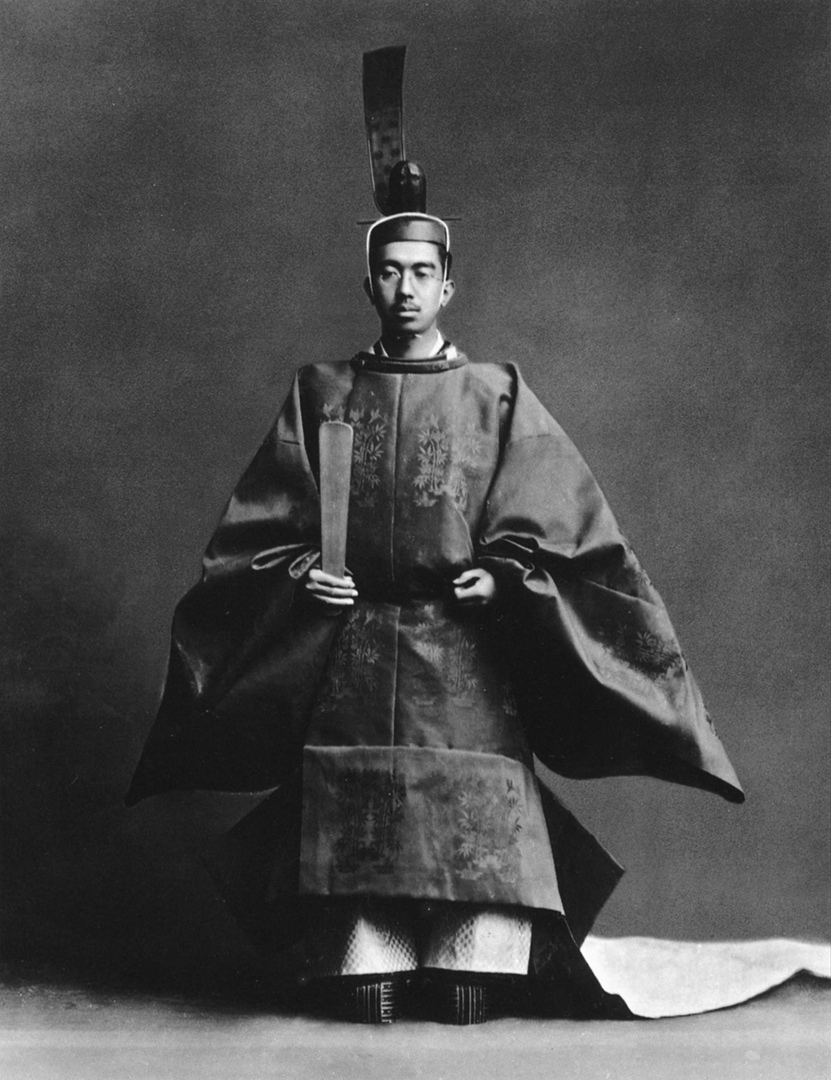
\includegraphics[scale=0.3]{Glava7/PGo8ZLKXlk4.jpg}
	%	\label{fig:scipion} % Unique label used for referencing the figure in-text\end{document}
	%	%\addcontentsline{toc}{figure}{Figure \ref{fig:placeholder}} % Uncomment to add the figure to the table of contents%----------------------------------------------------------------------------------------
	\caption{Хирохито в традиционных церемониальных одеяниях, 1928 год.}%	CHAPTER 2
\end{figure}

Он был молод, хорошо образован, успел обзавестись супругой - 26 января 1924 года Хирохито женился на своей дальней родственнице принцессе Нагако, и дочерью – маленькая принцесса Тэру родилась 9 декабря 1925. Новый монарх, как казалось, обещал новую надежду для государства. Никто ещё не знал, что именно в эпоху Сёва Япония вступит в самую тяжёлую войну в своей истории – и проиграет её…

О второй половине 1920-х, личности и первых шагах императора, армии и флоте, а также о влиянии на судьбу Японии мирового экономического кризиса – в следующей части. 

\url{https://vk.com/wall-162479647_83724}